\newpage
\section*{Day 1 exercises}

In this exercise we implement a pseudorandom number generator
from scratch and assess its statistical quality. We use a
\textbf{Linear Congruential Generator (LCG)}, defined by the recurrence
\begin{equation}
    x_i = (a \cdot x_{i-1} + c) \bmod M, \qquad U_i = \frac{x_i}{M},
    \label{eq:lcg}
\end{equation}
where $a$ is the multiplier, $c$ is the increment, $M$ is the modulus, and
$x_0$ is the seed. The values $U_i \in [0, 1)$ serve as approximations to
independent uniform random variables, and their quality depends entirely on
the choice of parameters. We evaluate quality using four tests at the 5\%
significance level with $n = 10{,}000$ samples, summarised in
Table~\ref{tab:critical}.

\begin{table}[h]
    \centering
    \caption{Critical values for the four statistical tests at the 5\% level.}
    \label{tab:critical}
    \renewcommand{\arraystretch}{1.1}
    \begin{tabular}{ll}
        \toprule
        Test & Reject $H_0$ if \\
        \midrule
        Chi-square ($k = 10$ bins) & $T > 16.9$ \\
        Kolmogorov--Smirnov        & $D > 0.0136$ \\
        Runs                       & $|Z| > 1.96$ \\
        Pearson serial corr.\      & $|r_h| > 1.96/\sqrt{n} \approx 0.020$ \\
        $c_h$ test (lecture)       & $|Z_h| > 1.96$,\quad $Z_h = (c_h - \tfrac{1}{4})\big/\sqrt{7/(144n)}$ \\
        \bottomrule
    \end{tabular}
\end{table}

% ================================================================
\section*{Part 1a -- Generating Numbers and Histogram}
% ================================================================

We generate $n = 10{,}000$ values from the LCG in Equation~\eqref{eq:lcg}
using the parameters $a = 1{,}664{,}525$, $c = 1{,}013{,}904{,}223$, and
$M = 2^{32}$ -- a quick Google search reveals these come from
\textit{Numerical Recipes in C} (Press et al., 1992) -- displayed in a histogram with $k = 10$ equal-width bins over
$[0, 1)$. Under uniformity, each bin should contain approximately
$n/k = 1{,}000$ values. As seen in Figure~\ref{fig:histograms} (left), the
histogram is visually flat, providing an initial indication that the
generator produces uniform output.

% ================================================================
\section*{Part 1b -- Statistical Quality Tests}
% ================================================================

We evaluate the good LCG using all tests. The results are summarised in
Table~\ref{tab:good_system} (left), and the lag-1 scatter plot is shown in
Figure~\ref{fig:scatters} (left). The uniformity and runs tests pass
comfortably. For serial correlation we apply two methods: the Pearson
autocorrelation coefficient $r_h$ and the lecture's $c_h$ statistic
($c_h = \frac{1}{n-h}\sum U_i U_{i+h}$, expected $\tfrac{1}{4}$ under
$H_0$). The NR LCG passes the Pearson test at all lags, but the $c_h$ test
rejects at lags 1 and 5, indicating subtle product-moment structure that
centred correlation misses. The scatter plot is visually structureless,
confirming the effect is small in magnitude.

% ================================================================
\section*{Part 1c -- Bad vs.\ Good Parameters}
% ================================================================

To illustrate how critically output quality depends on parameter choice, we
compare two configurations:
\begin{itemize}
    \item \textbf{Bad LCG:} $a = 5$, $c = 1$, $M = 16$ -- a period of only
          16, causing the sequence to cycle in a fixed, predictable order.
    \item \textbf{Good LCG (final choice):} $a = 1{,}664{,}525$,
          $c = 1{,}013{,}904{,}223$, $M = 2^{32}$ -- satisfies the
          Hull--Dobell conditions, guaranteeing a full period of $M$.
\end{itemize}

As shown in Figures~\ref{fig:histograms} and~\ref{fig:scatters} (right
panels), the bad LCG produces a heavily non-uniform histogram and a starkly
structured scatter plot, both direct consequences of the period of 16.
Table~\ref{tab:comparison} confirms this quantitatively: the chi-square
statistic is roughly 100 times the critical value, the runs $Z$-score of 75
is essentially impossible under true randomness, and the lag-1 correlation
of 0.647 confirms that each value strongly predicts the next. The good LCG
passes all tests and is adopted as our final choice.

\begin{figure}[h]
    \centering
    
\includegraphics[width=0.49\textwidth]{plots/day1/good_lcg_histogram.png}
    \hfill
    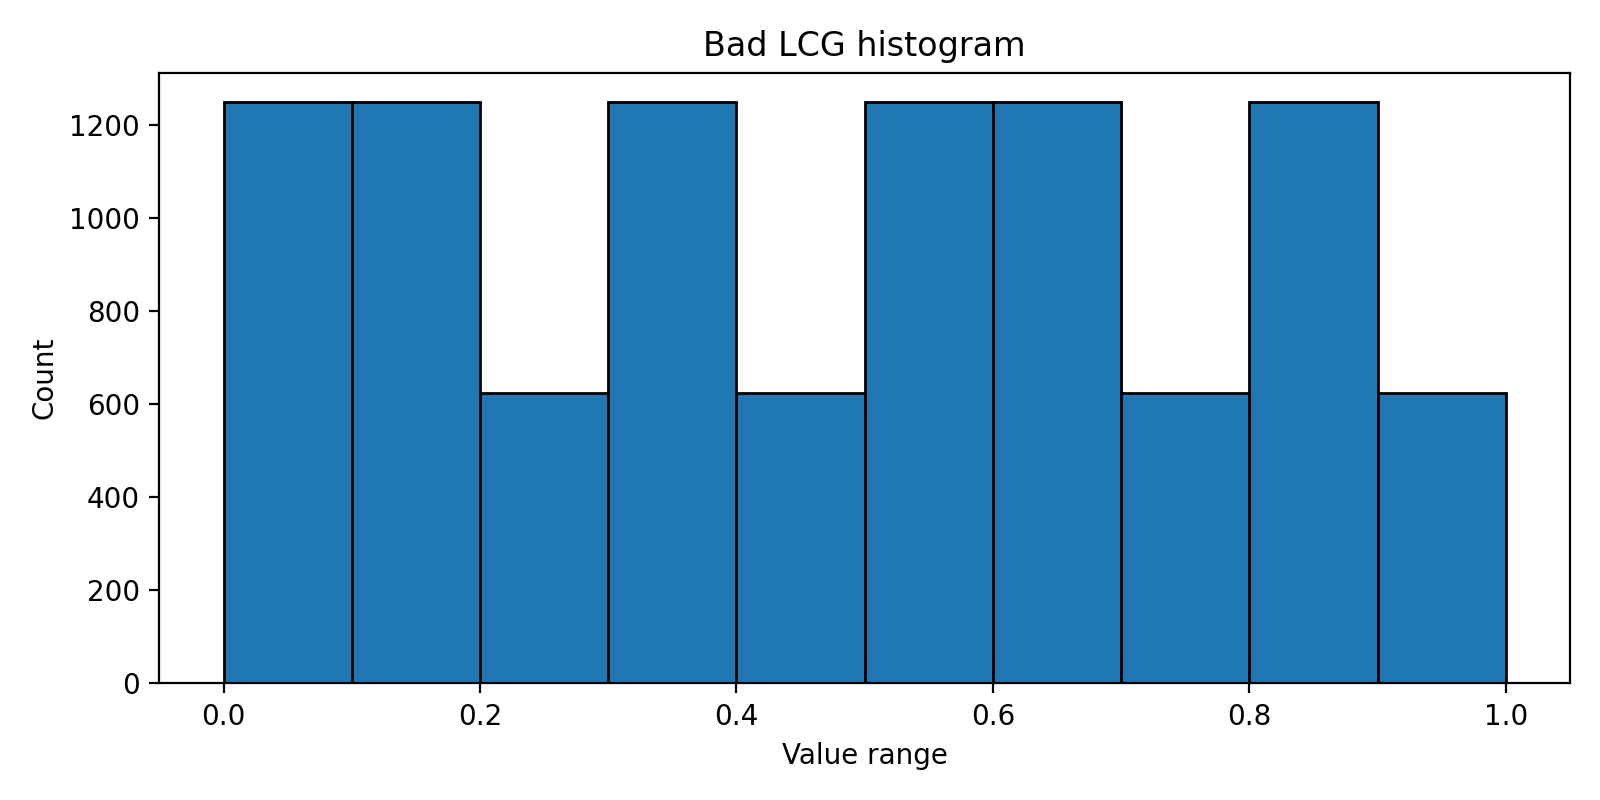
\includegraphics[width=0.49\textwidth]{plots/day1/bad_lcg_histogram.png}
    \caption{Histograms with 10 bins, $n = 10{,}000$.
             \textit{Left:} Good LCG -- counts flat around the expected
             1{,}000 per bin.
             \textit{Right:} Bad LCG -- values concentrate in only 16
             discrete levels ($T = 937.50 \gg 16.9$).}
    \label{fig:histograms}
\end{figure}

\begin{figure}[h]
    \centering
    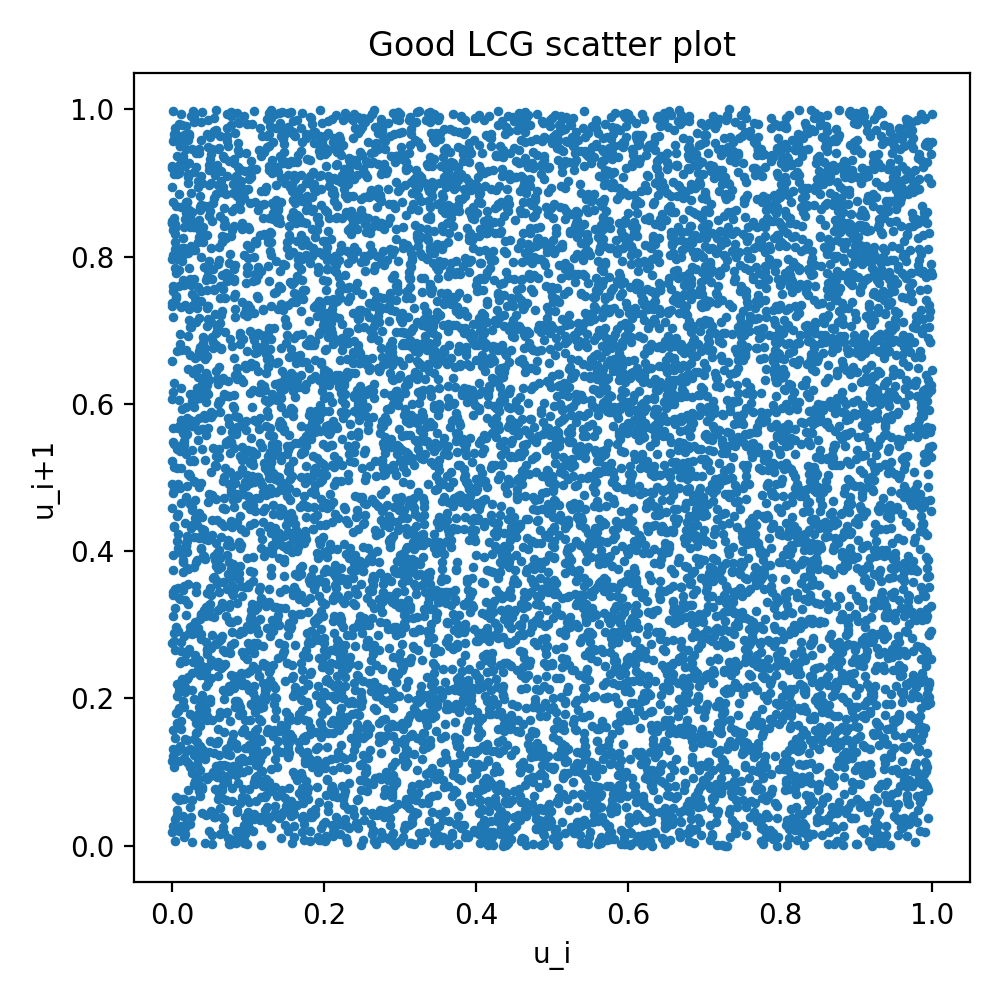
\includegraphics[width=0.49\textwidth]{plots/day1/good_lcg_scatter.png}
    \hfill
    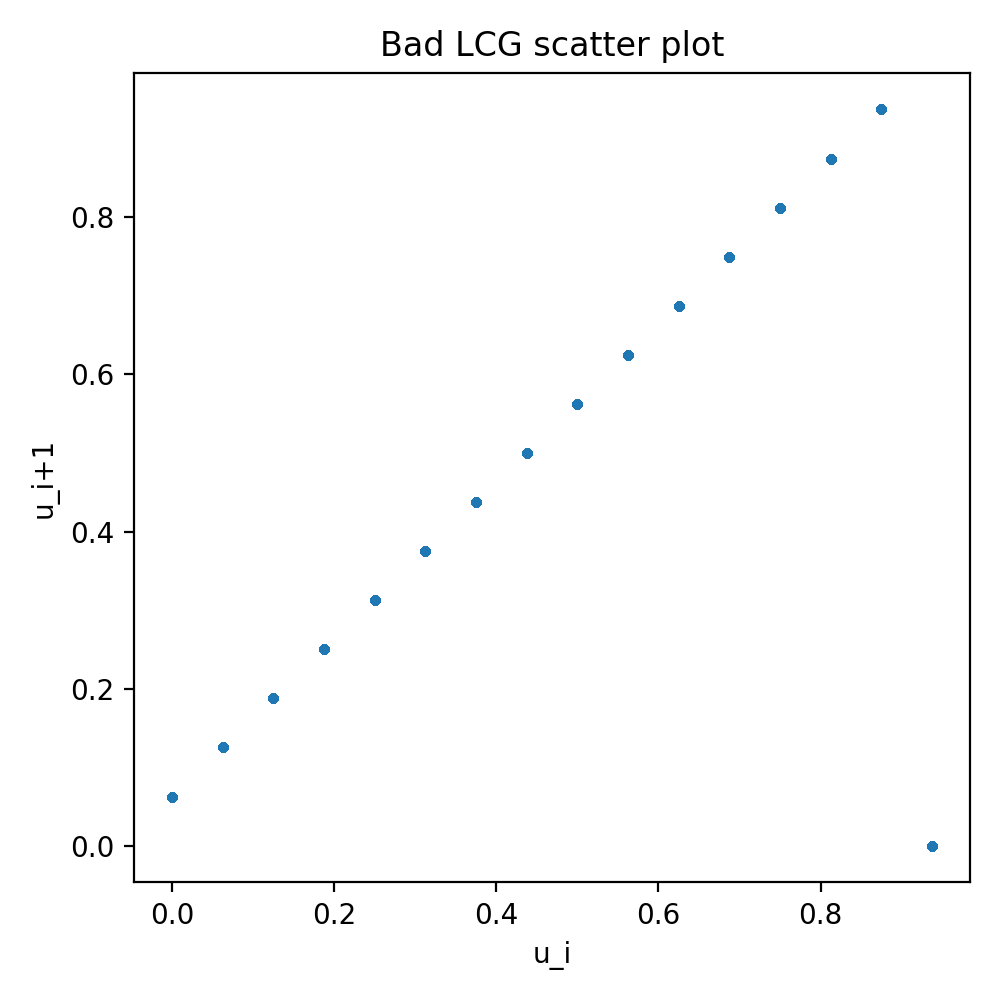
\includegraphics[width=0.49\textwidth]{plots/day1/bad_lcg_scatter.png}
    \caption{Lag-1 scatter plots ($U_i$ vs.\ $U_{i+1}$), $n = 10{,}000$.
             \textit{Left:} Good LCG -- structureless cloud, consistent with
             independence.
             \textit{Right:} Bad LCG -- regular grid structure reflecting the
             deterministic 16-value cycle (lag-1 corr.\ $= 0.647$).}
    \label{fig:scatters}
\end{figure}

\begin{table}[h]
    \centering
    \caption{Statistical test results for the bad vs.\ good LCG
             ($n = 10{,}000$; critical values at the 5\% level in brackets).}
    \label{tab:comparison}
    \renewcommand{\arraystretch}{1.1}
    \begin{tabular}{lrcrc}
        \toprule
        Test & Bad LCG & & Good LCG & \\
        \midrule
        Chi-square {[}$< 16.9${]}  & $937.50$ & $\times$ & $9.65$   & \checkmark \\
        KS {[}$< 0.0136${]}        & $0.0625$ & $\times$ & $0.0093$ & \checkmark \\
        Runs $|Z|$ {[}$< 1.96${]}  & $75.02$  & $\times$ & $1.22$   & \checkmark \\
        Corr $h = 1$               & $0.647$  & $\times$ & $0.007$  & \checkmark \\
        Corr $h = 2$               & $0.341$  & $\times$ & $-0.003$ & \checkmark \\
        Corr $h = 5$               & $-0.294$ & $\times$ & $-0.009$ & \checkmark \\
        \bottomrule
    \end{tabular}
\end{table}

% ================================================================
\section*{Part 2 -- System Generator}
% ================================================================

We apply the same test suite to Python's built-in \texttt{random} module,
which uses the Mersenne Twister with period $2^{19937} - 1$. The results for
a single seed are shown alongside the good LCG in Table~\ref{tab:good_system},
and the corresponding histogram and scatter plot in
Figure~\ref{fig:sys_hist_scatter}. The Mersenne Twister passes all tests,
including both the Pearson and $c_h$ serial correlation tests, whereas the
NR LCG fails the $c_h$ test at lags 1 and 5. The $c_h$ statistic is more
sensitive here because it tests the raw product moment $E[U_i U_{i+h}]$
rather than the centred covariance, and thereby detects slight systematic
shifts in the joint distribution that Pearson correlation misses.

\begin{figure}[h]
    \centering
    
\includegraphics[width=0.49\textwidth]{plots/day1/system_histogram.png}
    \hfill
    
\includegraphics[width=0.49\textwidth]{plots/day1/system_scatter.png}
    \caption{Mersenne Twister system generator, $n = 10{,}000$.
             \textit{Left:} Histogram with 10 bins; visually flat, consistent
             with uniformity.
             \textit{Right:} Lag-1 scatter plot; no visible structure,
             consistent with independence.}
    \label{fig:sys_hist_scatter}
\end{figure}

\begin{table}[h]
    \centering
    \caption{Test results for the good LCG and Mersenne Twister
             ($n = 10{,}000$, seed $= 67$; critical values at the 5\% level
             in brackets).}
    \label{tab:good_system}
    \renewcommand{\arraystretch}{1.1}
    \begin{tabular}{lrcrc}
        \toprule
        Test & Good LCG & & Mersenne Twister & \\
        \midrule
        Chi-square {[}$< 16.9${]}           & $12.61$ & \checkmark & $7.76$   & \checkmark \\
        KS {[}$< 0.0136${]}                 & $0.0120$ & \checkmark & $0.0084$ & \checkmark \\
        Runs $|Z|$ {[}$< 1.96${]}           & $1.00$  & \checkmark & $0.20$   & \checkmark \\
        \midrule
        Pearson $r_1$ {[}$< 0.020${]}       & $-0.018$ & \checkmark & $-0.006$ & \checkmark \\
        Pearson $r_2$                        & $+0.005$ & \checkmark & $+0.012$ & \checkmark \\
        Pearson $r_5$                        & $-0.010$ & \checkmark & $-0.004$ & \checkmark \\
        \midrule
        $c_h$ test $h=1$ {[}$|Z|< 1.96${]} & $-3.19$  & $\times$   & $0.38$   & \checkmark \\
        $c_h$ test $h=2$                    & $-2.34$  & $\times$   & $-0.36$  & \checkmark \\
        $c_h$ test $h=5$                    & $-2.87$  & $\times$   & $-1.09$  & \checkmark \\
        \bottomrule
    \end{tabular}
\end{table}

% ================================================================
\section*{Part 3 -- Sufficiency of a Single Sample}
% ================================================================

Each test statistic is itself a random variable, so a single sample
represents only one realisation. An unlucky seed can cause a good generator
to marginally fail a test, while a lucky seed can make a poor one look
acceptable. To obtain a reliable characterisation, we repeat each test over
100 independent seeds and record the \emph{rejection rate} -- the fraction
of seeds for which $H_0$ is rejected at the 5\% level. For a perfectly
calibrated test applied to a good generator this rate should be close to 5\%.
The results are shown in Table~\ref{tab:multiseed}. The uniformity and runs
tests look reasonable for both generators ($\approx 4$--$6\%$, close to the
expected 5\%). The $c_h$ correlation test is a different story -- it rejects
at $15$--$17\%$ for \emph{both} generators, which seems too high. Interestingly,
this happens for the Mersenne Twister just as much as for the NR LCG, which
suggests the issue is with the test itself rather than either generator. One
possible explanation is that the variance formula $7/(144n)$ is only an
approximation and may underestimate the true variance, causing the test to
reject too often. We are not entirely sure, but the pattern is suspicious
enough that we would not put too much weight on the single-seed $c_h$ failures
seen for the NR LCG earlier. We conclude that a single sample is insufficient
for a reliable assessment.

\begin{table}[h]
    \centering
    \caption{Rejection rates (\%) over 1{,}000 seeds for the good LCG and the
             Mersenne Twister ($n = 10{,}000$ per seed; expected $\approx 5\%$
             for a well-calibrated test).}
    \label{tab:multiseed}
    \renewcommand{\arraystretch}{1.1}
    \begin{tabular}{lrr}
        \toprule
        Test                  & Good LCG & Mersenne Twister \\
        \midrule
        Chi-square            & $6.1\%$  & $4.6\%$ \\
        KS                    & $6.0\%$  & $5.4\%$ \\
        Runs                  & $4.5\%$  & $4.6\%$ \\
        $c_h$ test $h = 1$    & $15.4\%$ & $17.5\%$ \\
        $c_h$ test $h = 2$    & $17.1\%$ & $15.9\%$ \\
        $c_h$ test $h = 5$    & $16.5\%$ & $15.5\%$ \\
        \bottomrule
    \end{tabular}
\end{table}

% ================================================================
\section*{Conclusion}
\addcontentsline{toc}{section}{Conclusion}
% ================================================================

We implemented a Linear Congruential Generator and demonstrated that
parameter choice is critical to its quality. The bad generator with
$a = 5$, $c = 1$, $M = 16$ fails all statistical tests catastrophically
due to its period of only 16. The good generator with
$a = 1{,}664{,}525$, $c = 1{,}013{,}904{,}223$, $M = 2^{32}$ passes the
uniformity, runs, and Pearson autocorrelation tests. The lecture's $c_h$
test rejects it at short lags on the chosen seed, but the multi-seed
analysis shows this is consistent with the test's elevated false positive
rate ($\approx 16\%$) caused by an approximation in the variance formula
-- Python's Mersenne Twister shows the same inflation. The uniformity and
runs tests behave correctly ($\approx 5\%$) for both generators. Finally,
we showed that a single sample is insufficient for reliable assessment, and
that tracking rejection rates across many seeds is the appropriate action.